% !TeX root = ../main-paper.tex
\section{Experimental Setup}


\begin{figure}[tb]
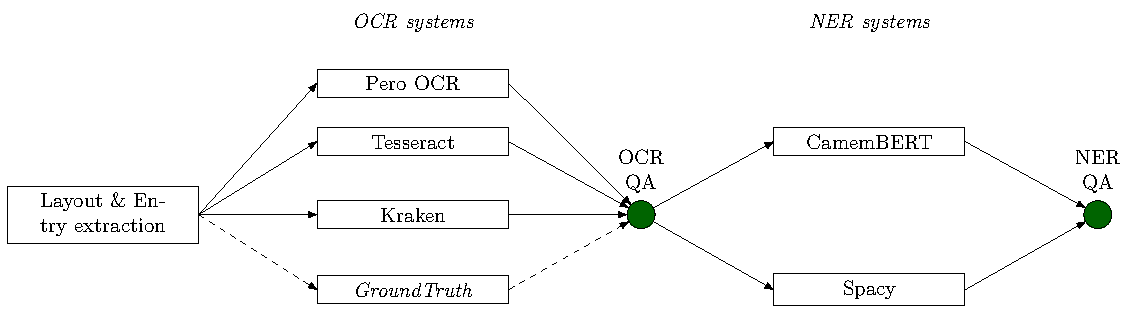
\includegraphics[width=\linewidth]{figs/protocol.pdf}
\caption{Scheme of the evaluation protocol.}
\label{fig.protocol}
\end{figure}

\subsection{Evaluation protocol \& Metrics}

\Cref{fig.protocol} depicts the evaluation procotol used to assess the OCR and NER systems. Two quality evaluation
are performed in the pipeline named respectively \emph{OCR Q.A.} and \emph{NER Q.A.}.

First the layout extraction and the entry segmentation of the page are performed with a semi-automated system and
checked by a human. Afterward, an OCR system runs on the thumbnails of each segmented entry to extract its text. An
entry might span over multiple text lines but is always single-block. Thus, the most adapted mode is chosen when
the OCR system allows for detection mode (e.g. the \emph{block} mode for \emph{Tesseract}). 

\textbf{OCR Q.A.} is performed after some text normalization of the OCR system outputs. Text normalization consists in
projecting unicode characters onto the latin-1 charset (whenever it makes sense) and removing extra symbols (hands,
crosses). Then, the predicted text is aligned with the reference text using standard tools and the Character Error Rates
(CER) are computed at entry level and at global level. 

\begin{align}
\mathrm{CER} &=  \frac{\#Errors}{\text{Reference Text Length}} & & \mathrm{CER}_\mathrm{norm} =  \frac{\#Errors}{\text{Alignment Length}} 
\end{align}

In this benchmark, we consider 3 OCR systems well-known for the historical document analysis: Pero OCR, Tesseract and Kraken. 

\edwin{FIXME: add ref papier eval OCR + ISRI, eval KRAKEN}


Next, a NER system extracts the named entities from the text of each entry outputed by the OCR and the \textbf{NER Q.A.}
is performed. The NER system outputs a text with tags that enclose the entities. To assess the quality of the entity
extraction, we rely on the same technique as for the OCR evaluation. The predicted text is aligned with the reference
text and the tags are projected in the alignment. Then, the CER \nathalie{non ici ce sont la précision, le rappel et la F-mesure qui sont calculées} is computed between each entity of the alignment and the
groundtruth as illustrated on \cref{fig.eval-ocr-ner}.

\subsection{Experiment 1: NER sensibility to the number of training samples}
The first experiment evaluates the performances of the three models on training sets of different sizes.
To do so, we split the gold reference into a training set, a development set, and a test set. The training set is then gradually reduced in size while maintaining the relative frequency of directories within.
The training and testing procedure is the same for the three models.

As the form and structure of entries varies across directory collections and through time, the model may learn to overfit on a subset of directories with specific features.
To reduce the evaluation bias, we start by leaving out 3 directories (1690 entries, ~20\%) from the gold reference to test each model on unseen directories.
Then a stratified sampling based on the entry directory name is applied to the remaining set to create a training (6373 entries, ~71\% of the gold reference) and a development set (709 entries, ~8\%).
This sampling procedure is a convenient way to shape both sets to reflect the diversity of directories within the gold reference.

To generate smaller training sets we start from the initial training set and attractively split it in half using the same stratified sampling strategy.
We stop if there is only one entry left in a directory or if the current train set contains less than 30 entries.
Applying this procedure to the initial training set produced 8 training sets containing 49, 99, 199, 398, 796, 1593, 3186 and 6373 entries.

% Move to metrics ?
All metrics are evaluated on the test set, yet the biased model performances on the development sets are add in the paper material as additional information.


\subsection{Experiment 2: NER in the presence of noisy OCR texts}

\begin{itemize}
\item At least 1 run per dataset, more if possible.
\item Only use the best model; should be CamemBERT+pretrained
\item Train on reference gold, evaluate on reference gold AND ocr-gold (2 datasets)
\item split train/dev/test the same way than experiment 1. Use the exact same splitting for datasets so the clean test set, pero test set and tesseract test sets contains the same entries.
\end{itemize}
 
 
%\begin{itemize}
%\item All : leave out 3 directories (~20\% of the dataset) as test data. Then apply stratified sampling based on the directory of each entry to split the remaining into a train set (~72\%) and a dev set (~8\%).
%\item Spacy CNN : No limit on epochs, instead use patience 1600.
%\item CamemBERT: 3 epochs.
%\item CamemBERT pretrained: 3 epochs, pretraining on MLM + NSP with ~20000 raw texts extracted with Pero-OCR.
%\end{itemize}



\subsection{Parameters for each method}

\subsection{OCR systems}
\begin{itemize}
    \item original OCR
    \item Tesseract 4
    \item Pero
    \item other?
\end{itemize}

\subsection{Implementation details}
We use Spacy\mcite{spacy} for the CNN implementation
and Huggingface for the BERT 
tok2vec(words embeddings + encoding) + attention layer  +  transition-based model.

\paragraph{Huggingface CamemBERT}
CamemBERT + linear classifier as decision layer



we use spacy  for the CNN implementation and Huggingface for BERT.

will we use FLAIR as well? $\rightarrow$ No